\section{Simulation}
\label{sec:simulation}

The study uses the synthetic susceptible-infected-removed mechanism of Section 4.1 of \citet{whitaker2025}, observed at spacings 1, 2 and 5. Spacing 1 is the published grid. Spacings 2 and 5 are coarser, and they were fixed before any weight was seen. All algorithms were coded in R. No processor is recorded for this run. The data are simulated. There is no gold-standard posterior: the diagnostic does not estimate a posterior distribution of the static parameters.

We drew 20 replicates, with 500 proposals in each window, from seed base 20251015. The seeds are a property of the study script, not of the guide. No fine-grid path was discarded. The run took 46.879 seconds. That time is a record of this run. It is not a comparison with the run times in \citet{whitaker2025}.

For each replicate, each spacing and each guide, the within-replicate summary is the median of the window values of Equation~\eqref{eq:ess}. The study summary is the median of those 20 numbers. The prediction uses the linear guide only. The myopic guide is computed on the same simulated paths and the same observations, with independent Poisson draws. Table~\ref{tab:s1} reports the linear guide. Figure~\ref{fig:ess} plots those three medians and the three myopic medians given below. The myopic series in the figure is a comparator and is not the prediction.

\begin{table}[t]
\centering
\caption{Linear incidence guide. Median effective sample size across 20 replicates, reported to two decimal places. Finite-weight medians use the draws with a finite log weight. Myopic medians are given in Section~\ref{sec:simulation}.}
\label{tab:s1}
{\small\setlength{\tabcolsep}{3pt}%
\begin{tabular}{rrrr}
\hline
Spacing & ESS & ESS, finite weights & Invalid proportion \\
\hline
1 & 149.66 & 149.66 & 0.033 \\
2 & 8.09 & 8.09 & 0.009 \\
5 & 2.06 & 2.06 & 0 \\
\hline
\end{tabular}}
\end{table}


\begin{figure}[t]
\centering
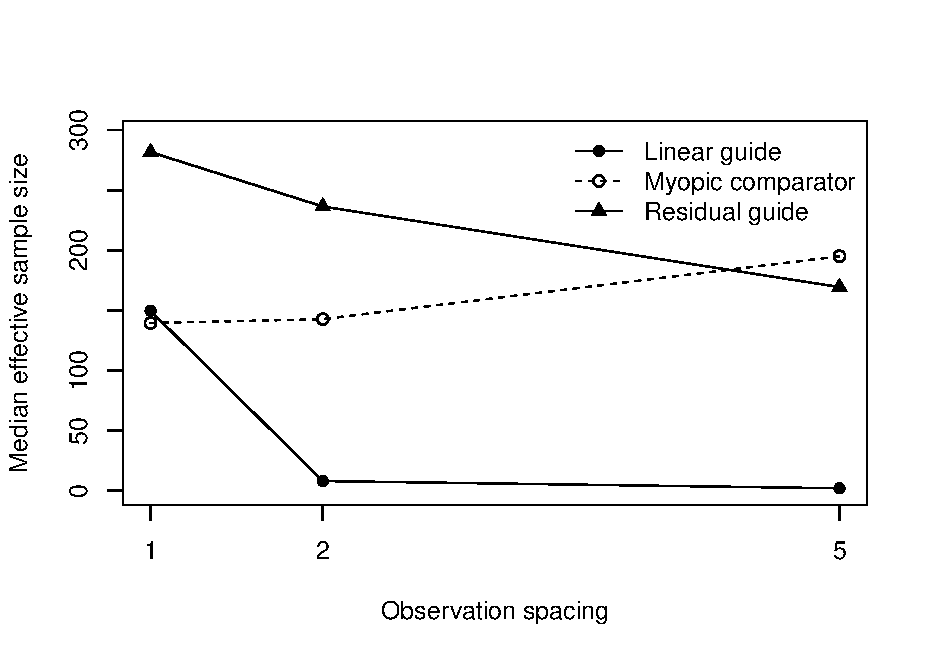
\includegraphics[width=0.72\textwidth]{figures/ess-against-spacing.pdf}
\caption{Effective sample size against observation spacing. Filled circles: linear guide, the medians in Table~\ref{tab:s1}. Open circles: myopic comparator, which is not the prediction. The myopic values are those stated in the text.}
\label{fig:ess}
\end{figure}

From Table~\ref{tab:s1}, the linear median effective sample size is 149.660679297905 at spacing 1 and 2.05670742297318 at spacing 5. The value at spacing 5 is smaller, so the prediction holds. At spacing 2 the linear median is 8.09166818813341. At every linear row, the median that includes zero weights equals the median computed on the finite weights alone. The fall is present in the finite weights. The median proportion of invalid draws is 0.0329 at spacing 1, 0.009 at spacing 2 and 0 at spacing 5, so the fall at spacing 5 is not produced by the zero-weight rule.

At spacing 1 the myopic median is 139.525563697813. At spacing 2 it is 142.824313796391. At spacing 5 it is 195.181391518181. The myopic median does not fall as the spacing grows.

Two qualifications belong with the comparison. The guide was given the simulated prevalence and the simulated contact-rate path. The result is about \(h^{*}\) given those paths. At spacing 1 the linear median is 149.660679297905 out of 500 draws, so the guide is already uneven on the published grid. The prediction was the comparison across spacings, not a claim that the published grid is unaffected. The comparison does not measure a pathwise distance to the true conditioned process, and it does not say whether a filtering distribution would change.
